\begin{figure}[!ht]
\centering
\subfigure[Usual\label{subfig:usual}]{
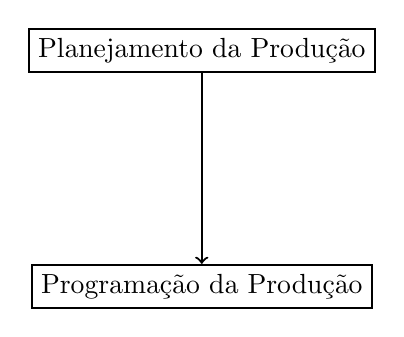
\begin{tikzpicture}
\node[draw, rectangle, thick] at (0,3) (plan) {Planejamento da Produção};
\node[draw, rectangle, thick] at (0,0) (prog) {Programação da Produção};
\draw [->, thick] (plan) -- (prog);
\end{tikzpicture}
}
\hspace{2cm}
\subfigure[Proposto\label{subfig:prop}]{
\begin{tikzpicture}
\node[draw, rectangle, thick] at (0,3) (plan) {Planejamento da Produção}
    edge[pil,bend left=45] (prog.east);
\node[draw, rectangle, thick] at (0,0) (prog) {Programação da Produção}
    edge[pil,bend left=45] (plan.west);
%\draw[->,thick] (plan) --(3,3) -- (3,0) -- (prog); \draw[->,thick] (prog) --(-3,0) -- (-3,3) -- (plan);
\end{tikzpicture}
}
\caption{Comparação das estruturas usual e proposta.}
\label{fig:plan_prog}
\end{figure}
